\chapter{需求建模 }
\section{数据流图}
\subsection{顶层数据流图}
\begin{figure}[ht]
\centering
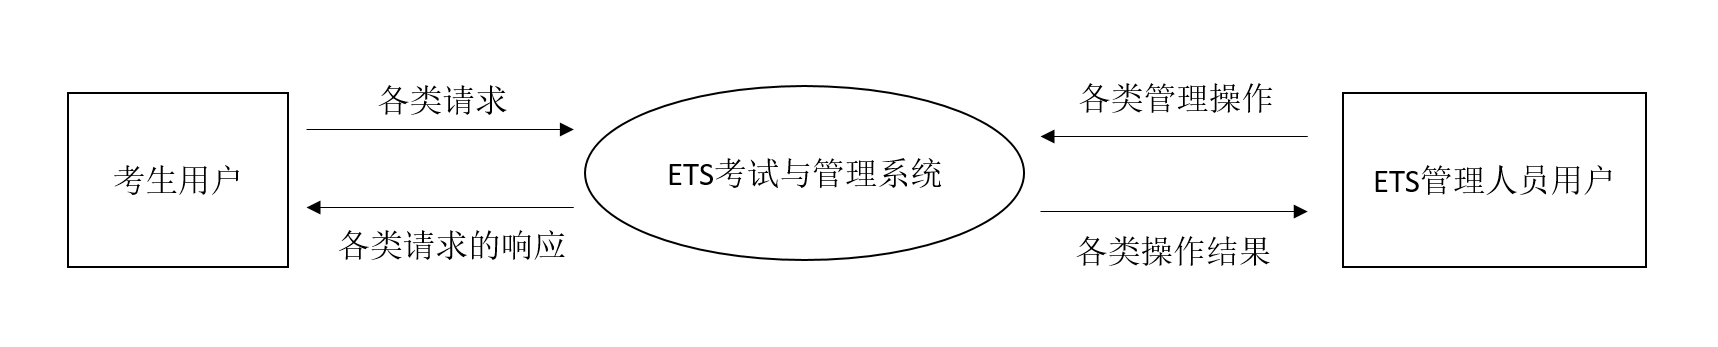
\includegraphics[width=15cm]{top_module.png}
\caption{顶层数据流图}\label{fig:noted-figure}
%\note{the solid lines represent the time histogram of the spontaneous activities of an old monkey cell(gray) and a young monkey cell (black). The bin-width is 1}
\end{figure}


\subsection{0层数据流图}
\begin{figure}[htb]
\centering
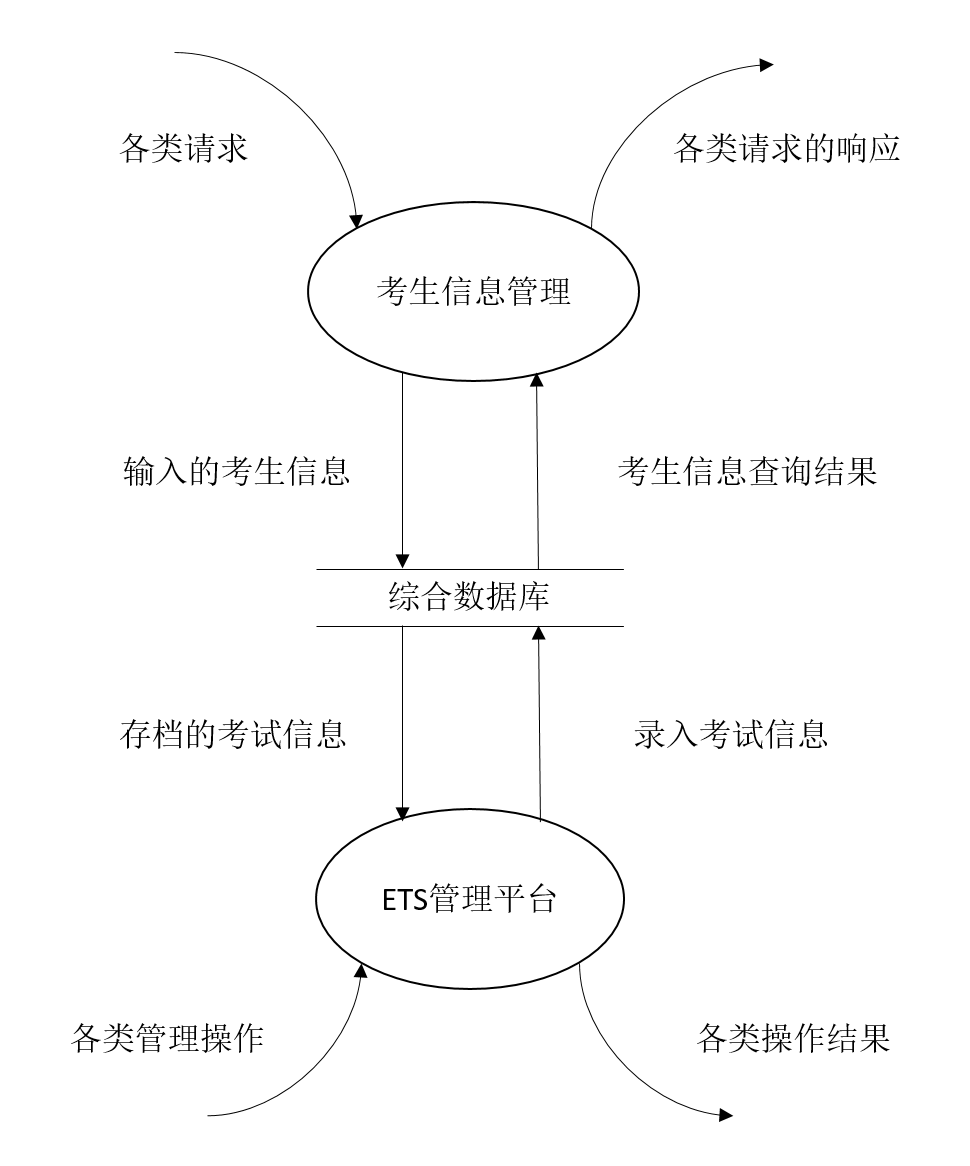
\includegraphics[width=8cm]{zero_module.png}
\caption{0层数据流图}\label{fig:noted-figure}
%\note{the solid lines represent the time histogram of the spontaneous activities of an old monkey cell(gray) and a young monkey cell (black). The bin-width is 1}
\end{figure}

\subsection{1层数据流图}
\begin{figure}[htb]
\centering
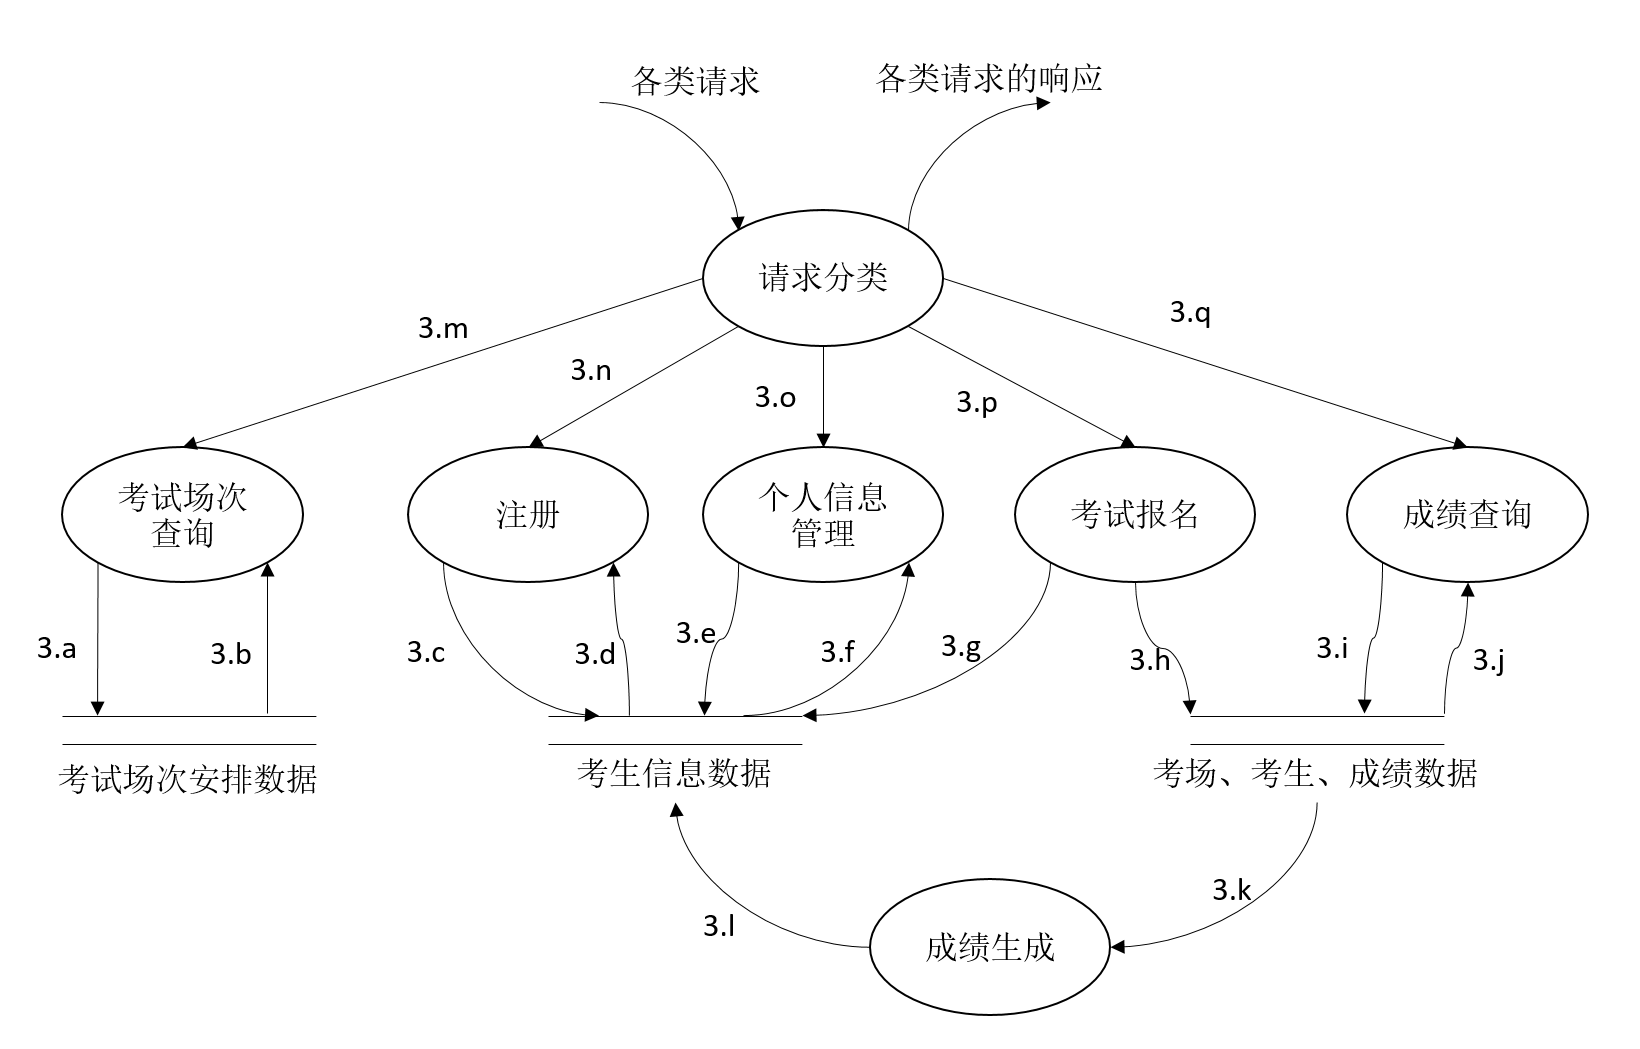
\includegraphics[width=10cm]{one_module.png}
\caption{考生用户子系统1层数据流图}\label{fig:noted-figure}
%\note{the solid lines represent the time histogram of the spontaneous activities of an old monkey cell(gray) and a young monkey cell (black). The bin-width is 1}
\end{figure}

\subsection{1层数据流图}
\begin{figure}[htb]
\centering
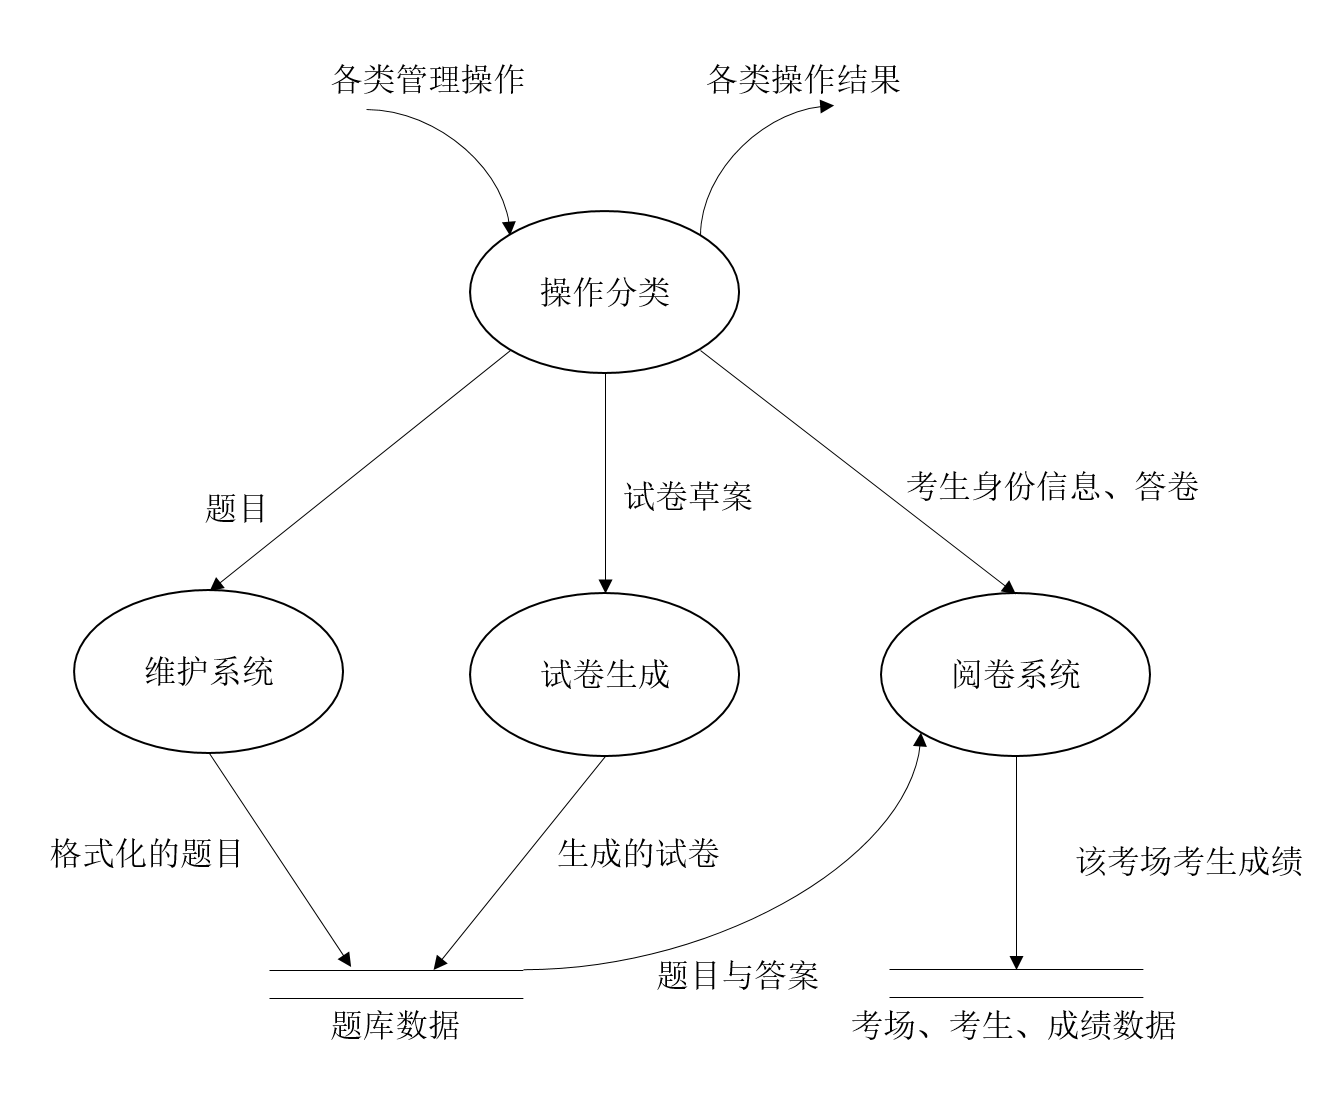
\includegraphics[width=10cm]{two_module.png}
\caption{ETS管理子系统1层数据流图}\label{fig:noted-figure}
%\note{the solid lines represent the time histogram of the spontaneous activities of an old monkey cell(gray) and a young monkey cell (black). The bin-width is 1}
\end{figure}

\section{数据字典}
\subsection{数据流说明}
(1)

名称:各类请求

描述:考生用户提交给系统的各类请求

来源:由考生用户提交

去处:由考生信息管理子系统处理

组成:包括新用户注册、个人信息查询、考试信息查询、预缴费、考试报名、成绩查询等。

(2)

名称:各类请求的响应

描述:系统返回给考生查询的信息

来源:考生信息管理系统

去处:提供给位于终端的考生用户

组成:取决于具体的请求,如成功存储的个人信息、考试时间地点信息等。

(3)

名称:各类管理操作

描述:ETS管理人员提交给系统进行的各类操作

来源:ETS管理员

去处:由考试管理子系统处理

组成:包括发布考试信息、试题维护、试卷成型等。

(4)

名称:各类操作结果

描述:系统返回给ETS管理人员的各类操作结果,如更新的试题等。

来源:考试管理子系统

去处:提交给ETS管理人员

(5)

名称:输入的考生信息

描述:需向数据库提交的查询或修改请求中包含的与该考生相关信息。

来源:考生信息管理系统的预处理结果

去处:存入考生信息数据库

(6)

名称:考生信息查询结果

描述:信息查询或修改完成后,数据库返回给考生信息管理子系统的结果。

来源:考生信息数据库

去处:给考生信息管理子系统处理

(7)

名称:存档的考试信息

描述:数据库向ETS管理平台子系统提供的已保存的考试信息。

来源:考试信息数据库

去处:供考试管理子系统使用

(8)

名称:录入考试信息

描述:ETS管理平台子系统向数据库写入的更新考试信息。

来源:考试管理系统对考试信息的处理结果

去处:存入考试信息数据库

(9)

编号:3.a

名称:考试场次安排查询

描述:全年考试时间地点安排或考位查询。

来源:考试场次查询过程

去处:记录考试场次信息的数据库

(10)

编号:3.b

名称:考试场次安排查询结果

描述:全年考试时间地点安排或考位情况。

来源:记录考试场次信息的数据库

去处:给考生信息管理子系统处理的请求结果

(11)

编号:3.c

名称:注册信息

描述:新用户注册时输入的信息。

来源:注册过程

去处:记录考生信息的数据库

(12)

编号:3.d

名称:注册结果

描述:写入数据库的注册信息。

来源:记录考生信息的数据库

去处:给考生信息管理子系统处理的请求结果

(13)

编号:3.e

名称:个人信息查询请求

描述:考生信息管理子系统提交给考生信息数据库的用户个人信息查询请求。

来源:个人信息管理过程

去处:记录考生信息的数据库

(14)

编号:3.f

名称:个人信息查询结果

描述:考生信息数据库返回给考生信息管理子系统的用户个人信息。

来源:记录考生信息的数据库

去处:给考生信息管理子系统处理的请求结果

(15)

编号:3.g

名称:考试报名信息

描述:考生信息管理子系统提交给考生信息数据库的考试报名信息。

来源:考试报名过程

去处:记录考生信息的数据库

(16)

编号:3.h

名称:考试报名信息

描述:考生信息管理子系统提交给考场、考生、成绩数据库的考试报名信息。

来源:考试报名过程

去处:记录考生考试注册信息的数据库

(17)

编号:3.i

名称:成绩查询请求

描述:考生信息管理子系统提交给考场、考生、成绩数据库的成绩查询请求,包括了用户信息。

来源:成绩查询过程

去处:记录考生已参加考试及成绩信息的数据库

(18)

编号:3.j

名称:成绩查询结果

描述:考场、考生、成绩数据库提交给考生信息管理子系统的成绩信息。

来源:记录考生已参加考试及成绩信息的数据库

去处:给考生信息管理子系统处理的请求结果

(19)

编号:3.k

名称:考生成绩

描述:从考场、考生、成绩数据库提取的考生成绩

来源:记录考生已参加考试及成绩信息的数据库

去处:成绩生成过程

(20)

编号:3.l

名称:考生成绩

描述:成绩生成过程写入考生信息数据库的考生成绩

来源:成绩生成过程

去处:记录考生信息的数据库

(21)

编号:3.m

名称:考试场次查询请求

来源:请求分类过程

去处:考试场次查询过程

(22)

编号:3.n

名称:注册请求

来源:请求分类过程

去处:注册过程

(23)

编号:3.o

名称:个人信息查询、更新请求

来源:请求分类过程

去处:个人信息管理过程

(24)

编号:3.p

名称:考试报名请求

来源:请求分类过程

去处:考试报名过程

(25)

编号:3.q

名称:成绩查询请求

来源:请求分类过程

去处:成绩查询过程

(26)

名称:题目

描述:ETS管理员需添加到题库的题目。

来源:操作分类过程

去处:题库维护过程

(27)

名称:格式化的题目

描述:经题库维护系统格式化后写入题库数据库的题目。

来源:题库维护过程

去处:题库数据库

(28)

名称:试卷草案

描述:ETS管理员需添加的一套试题材料。

来源:操作分类过程

去处:试卷生成过程

(29)

名称:生成的试卷

描述:经试卷生成模块生成的格式化试卷。

来源:试卷生成过程

去处:题库数据库

(30)

名称:考生身份信息、答卷

描述:参加一场考试的考生的身份信息与与之关联的答卷。

来源:操作分类过程

去处:阅卷系统

(31)

名称:题目与答案

描述:从题库数据库得到的试卷与标准答案。

来源:题库数据库

去处:阅卷系统

(32)

名称:该考场考生成绩

描述:写入考场、考生、成绩数据库的参加一场考试的考生成绩。

来源:阅卷系统

去处:记录考生成绩的数据库

\subsection{数据存储说明}
(1)

名称:综合数据库

描述:系统使用到的各个数据库的统称。

(2)

名称:考试场次安排

描述:记录各考场的考试时间安排及考位信息。

(3)

名称:考生信息

描述:记录与每个考生用户相关的信息,包括基本信息、已报名考试信息、成绩等。

(4)

名称:考场、考生、成绩数据

描述:记录参加一场考试的考生的成绩。

(5)

名称:题库数据

描述:记录题库及标准答案。


\subsection{加工说明}
(1)

名称:ETS考试与管理系统

描述:ETS考试与管理系统负责接受考生和ETS管理人员的请求,处理各个请求并且将请求反馈的信息传回给用户和ETS管理人员。

(2)

名称:考生信息管理

描述:考生信息管理系统负责接受考生的各类请求,例如缴费,更改密码,查阅考试成绩等。系统将会根据各类请求更新数据库,并且将对应的反馈信息传回给考生,例如考生的成绩以及考生是否缴费成功的信息等。

(3)

名称:ETS管理平台

描述:ETS管理平台负责接受ETS管理人员的各类请求,例如查看某一考生的具体信息,将考生成绩录入到系统中等。平台将根据各类请求向数据库发送查询或者修改请求,并且将对应的请求结果传回给ETS管理人员。

(4)

名称:请求分类

描述:负责将用户的各类输入请求进行分类以区分用户的具体要求,例如更改信息,查看成绩等。经过具体分类的请求将会传给下一层的不同加工体。

(5)

名称:考试场次查询

描述:该加工体负责接收考试场次查询的指令,向对应的数据库请求考试场次的信息,并且将对应的信息返回给用户。

(6)

名称:注册

描述:该加工体负责接收用户请求注册的信息和用户对应的注册信息,将注册信息写入考生信息管理数据库,并将操作成功与否的结果反馈给考生。

(7)

名称:个人信息管理

描述:该加工体负责接收用户请求查看用户资料的指令,并且向数据库发送查询请求来获得考生信息,并且将具体的信息重新反馈给考生。

(8)

名称:考试报名

描述:该加工体负责接收用户请求报名的指令,更改用户在考生信息数据库中是否已经报名考试的信息,并且将对应的信息写入到考场数据库中。

(9)

名称:成绩查询

描述:该加工体负责接收用户成绩查询指令。

(10)

名称:成绩生成

描述:该加工体负责将考场、考生、成绩数据库中按考场和考试场次组织的成绩转移到考生信息数据库中。

(11)

名称:操作分类

描述:该加工体负责将ETS管理人员的请求分类交给不同的加工体处理。

(12)

名称:维护系统

描述:该加工体接受ETS管理人员对题库的修改,维护题库完整正确。

(13)

名称:试卷生成

描述:该加工体接受ETS管理人员提供的组成试卷的材料,并合成一份试卷。

(14)

名称:阅卷系统

描述:该加工体接受试卷、考生答卷与标准答案,生成考生客观题成绩。
